\section{The orientifold index and the all-$d$ structure}\label{sec:index}

\subsection{Setup}\label{sec:index-setup}
Following \S3 of \cite{AgSc12}, M-theory on $\mathcal{X} \times \mathrm{TN} \times S^1$, with $\mathcal X$ the resolved conifold, is twisted by $(q, t)$. The orientifold action $\tilde I$ is the composition of an antiholomorphic involution $I$ of $\mathcal X$ with $z_2 \to -z_2$ in spacetime.
The probe of a knot $K$ is an M5-brane extended along the $z_2$ plane (a $t$-brane: the open-string denominator is $1/(1-t)$). On the cover there are two of them, $L_K$ and its image $I(L_K)$; see Figure \ref{fig:orientifold}.
The space of one-particle states on the cover is $H_1 = H_{\mathrm{int}} \otimes F_{z_2}$, where $F_{z_2}$ consists of the modes $t^l$, $l \ge 0$, in the $z_2$ direction, on which $\tilde I$ acts by $(-1)^l$. A \emph{sector} of the generating function is labelled by the numbers of boxes (total windings) on $L_K$ and on $I(L_K)$; a sector is \emph{fixed} when $\tilde I$ maps it to itself, i.e., when the two numbers are equal. States that exist only in the quotient, frozen at $z_2 = 0$ and wrapped on non-orientable surfaces, are called \emph{frozen states}.

\begin{figure}[htbp]
\centering
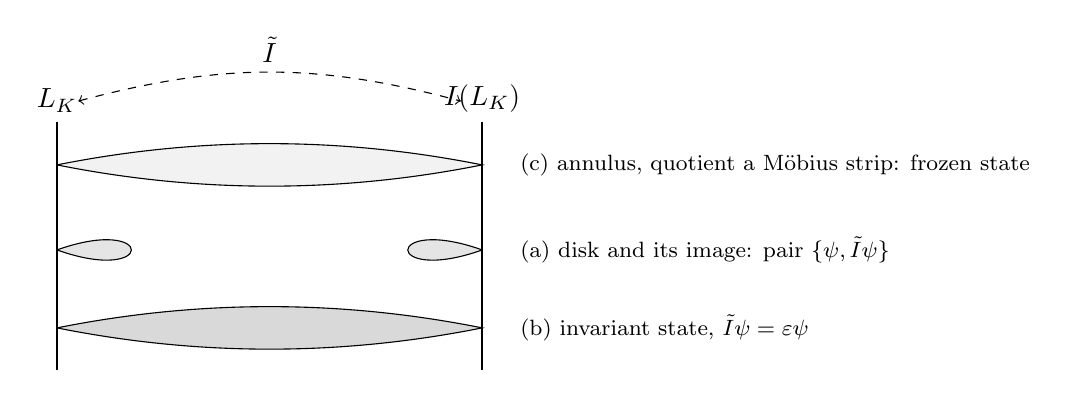
\begin{tikzpicture}[scale=0.9]
\draw[thick] (0,-0.3) -- (0,3.2) node[above] {$L_K$};
\draw[thick] (6,-0.3) -- (6,3.2) node[above] {$I(L_K)$};
\draw[<->,dashed] (0.3,3.5) to[bend left=15] node[midway,above] {$\tilde I$} (5.7,3.5);
% annulus between L and I(L): its quotient is a Moebius strip (frozen state)
\draw[fill=gray!10] (0,2.6) .. controls (2,3.0) and (4,3.0) .. (6,2.6) .. controls (4,2.2) and (2,2.2) .. (0,2.6);
\node[right] at (6.4,2.6) {\footnotesize (c) annulus, quotient a M\"obius strip: frozen state};
% pair: a disk on L_K and its image
\draw[fill=gray!20] (0,1.4) .. controls (1.4,1.9) and (1.4,0.9) .. (0,1.4);
\draw[fill=gray!20] (6,1.4) .. controls (4.6,1.9) and (4.6,0.9) .. (6,1.4);
\node[right] at (6.4,1.4) {\footnotesize (a) disk and its image: pair $\{\psi, \tilde I\psi\}$};
% invariant state: symmetric curve ending on both
\draw[fill=gray!30] (0,0.3) .. controls (2,-0.1) and (4,-0.1) .. (6,0.3) .. controls (4,0.7) and (2,0.7) .. (0,0.3);
\node[right] at (6.4,0.3) {\footnotesize (b) invariant state, $\tilde I\psi = \varepsilon\psi$};
\end{tikzpicture}
\caption{The cover with the brane $L_K$ and its image $I(L_K)$, and the three classes of one-particle states of Hypothesis \ref{hyp:classes}: pairs exchanged by $\tilde I$, states invariant under $\tilde I$ (in fixed sectors, with equal numbers of boundaries on $L_K$ and $I(L_K)$), and frozen states, whose world-sheets are quotients of surfaces connecting $L_K$ to $I(L_K)$ (an annulus becomes a M\"obius strip).}\label{fig:orientifold}
\end{figure}

\begin{hypothesis}[classification of one-particle states]\label{hyp:classes}
The one-particle states of the quotient are the $\tilde I$-orbits on the cover and fall into three classes:
\begin{enumerate}
\item pairs $\{\psi, \tilde I\psi\}$ exchanged by $\tilde I$, carrying the full tower of modes;
\item invariant states $\tilde I\psi = \varepsilon\psi$ ($\varepsilon = \pm 1$), carrying only the modes with $(-1)^l\varepsilon = 1$;
\item frozen states, carrying no tower of modes.
\end{enumerate}
This is the classification underlying the product formula (3.13) of \cite{AgSc12} for closed strings, extrapolated to open strings.
\end{hypothesis}

\subsection{All-$d$ structure}
% [O1][O2]
\begin{proposition}\label{prop:alld}
Under Hypothesis \ref{hyp:classes}, writing $\omega_\psi$ for the charge (the monomial in $q, t, \lambda$) of a state $\psi$,
\begin{equation}\label{eq:alld}
g = f - \tfrac12 f^{\cov} = \frac12\,\frac{E}{1+t} + C,\qquad E = \sum_{\text{invariant}} \varepsilon_\psi\, \omega_\psi,\qquad C = \sum_{\text{frozen}} \omega_\psi .
\end{equation}
\end{proposition}
\begin{proof}
The index of the cover is $f^{\cov} = \sum_{\text{pairs}} 2\omega/(1-t) + \sum_{\text{invariant}} \omega/(1-t)$, that of the quotient is $f = \sum_{\text{pairs}} \omega/(1-t) + \sum_{\text{invariant}} \omega \sum_{(-1)^l\varepsilon = 1} t^l + \sum_{\text{frozen}} \omega$. Substitute $\sum_{(-1)^l\varepsilon = 1} t^l = \tfrac12[1/(1-t) + \varepsilon/(1+t)]$.
\end{proof}

\begin{remark}\label{rem:Esector}
Invariant states exist only in fixed sectors; hence $E$ appears only there. If $\tilde I$ acts as the exchange of brane and image, its trace enters the power-sum basis in the $p_2$-type direction (the Adams operation $\psi^2$), and $E_{\ytwo} = -E_{\yoneone}$. The latter is verified for the Hopf link (Result \ref{cr:E22}) and for knots with two boxes (Result \ref{cr:largeN}).
\end{remark}

\begin{remark}[trace form]\label{rem:trace}
Equation \eqref{eq:alld} can be written as a trace: $f = \Tr_{H_1^{\cov}}(P_+\cdot) + C$ with the projection $P_+ = \tfrac12(1 + \tilde I)$, and $\Tr(\tilde I\cdot) = \sum_{\text{invariant}}\varepsilon\omega\sum_l(-t)^l = E/(1+t)$, so $g = \tfrac12\Tr_{H_1^{\cov}}(\tilde I\cdot) + C$. Thus $E$ is a twisted trace over the states of the cover and $C$ the contribution of states existing only in the quotient. This is the $\SO(2N)$ analogue of the two expressions given in \cite{Witten11} (\S3.4 there) for the Chern--Simons partition function of a non-simply-laced group: a trace with an outer automorphism inserted over the larger theory, and an ordinary trace over the fixed theory; the $D$-type $(2,0)$ theory arises there from M5-branes on $\mathcal X/\mathbb{Z}_2$ (\S5.1.4 of \cite{Witten11}, Appendix A of \cite{AgSc12}), which is the five-brane origin of $\tilde I$. The ambiguity of Proposition \ref{prop:EC} below is the ambiguity in splitting one number into these two expressions.
\end{remark}

\subsection{Action of $\tilde I$ on boundary zero modes}\label{sec:boundary}
In \S3.2 of \cite{KN17}, a holomorphic curve with $h$ boundaries carries boundary zero modes $d\theta_i$, $i = 1, \dots, h$, with the constraint $\sum_i d\theta_i = 0$; they span hook representations, and in the $t$-brane formulation each independent mode contributes a factor $(1 - q^{-1})$, which we normalize by $q^{1/2}$ to $z_q$.
% [O10]
\begin{proposition}\label{prop:boundary}
Assume the boundary zero mode picture of \cite{KN17} and let $\tilde I$ exchange the boundaries on $L_K$ with those on $I(L_K)$. A $\tilde I$-invariant curve lies in a fixed sector and has the same number $n$ of boundaries on $L_K$ and on $I(L_K)$, exchanged in pairs $(\theta_i, \theta_i')$. The sum $d\theta_i + d\theta_i'$ is $\tilde I$-even and the difference $d\theta_i - d\theta_i'$ is $\tilde I$-odd; the constraint $\sum d\theta = 0$ removes one even mode. In the trace with $\tilde I$ inserted an odd mode contributes $(1 + q^{-1})$ instead of $(1 - q^{-1})$. Hence
\begin{equation}\label{eq:boundary}
\text{boundary factor of } E = z_q^{\,n-1}(z_q^+)^{\,n},\qquad
\text{boundary factor of } \Phifix := (1-t)f^{\cov}\big|_{\text{fixed sector}} = z_q^{\,2n-1}.
\end{equation}
\end{proposition}
\begin{proof}
A curve whose numbers of boxes on $L_K$ and $I(L_K)$ differ is mapped by $\tilde I$ to a different sector and cannot be invariant; for an invariant curve $\tilde I$ maps boundaries on $L_K$ bijectively to boundaries on $I(L_K)$. Multiply $n-1$ even factors $(1 - q^{-1})$ and $n$ odd factors $(1 + q^{-1})$ for $E$, and $2n - 1$ factors $(1 - q^{-1})$ for $\Phifix$; the normalization by $q^{1/2}$ turns them into $z_q$ and $z_q^+$.
\end{proof}
The predictions are compared with the computations in Result \ref{cr:boundary}. What remains unknown is the action of $\tilde I$ on the moduli part $H^*(\mathcal{M}_{g,h,\beta})$, i.e., the sign $\varepsilon$ for each $\beta$.

\subsection{The \texorpdfstring{$E$--$C$}{E-C} ambiguity and the conditions fixing $E$}\label{sec:Econd}
% [O3]
\begin{proposition}\label{prop:EC}
For any integer Laurent polynomial $X$, the replacement $E \to E + 2(1+t)X$, $C \to C - X$ leaves $g$ unchanged. Hence $g$ determines only the class of $E$ modulo $2(1+t)$; in particular $E$ itself is not determined, while $E(-1) = [2(1+t)g]_{t=-1}$ is.
\end{proposition}
\begin{proof}
$\tfrac12 \cdot 2(1+t)X/(1+t) = X$, so the change of $E$ is compensated by that of $C$. In terms of states, the following two configurations are indistinguishable in both $f$ and $f^{\cov}$: a frozen state $\omega$ together with two pairs exchanged by $\tilde I$, one of charge $\omega$ and one of charge $\omega t$; and four invariant states $\omega, \omega, \omega t, \omega t$ with $\varepsilon = +1$. Both contribute $2(\omega + \omega t)/(1-t)$ to $f^{\cov}$ and $2\omega/(1-t)$ to $f$.
\end{proof}
% [O7]
\begin{corollary}\label{cor:Efree}
The $p_1^n$ directions of the power-sum basis and the sectors with an odd number of boxes (where $E = 0$) are independent of $E$. In these directions positivity can be tested independently of the $E$ ambiguity.
\end{corollary}

The definition $g^{\mathrm{odd}}$ of \cite{Marino09} with $\sum_{d\ \mathrm{odd}}$ is related to the all-$d$ definition as follows. Writing the oriented part with all $d$ and the crosscap part with odd $d$ only, as in \cite{Marino09}, and comparing with \eqref{eq:Z}, the terms with even $d$ of the all-$d$ expansion are accounted for by the Adams operation on $g^{\mathrm{odd}}$:
\begin{equation}\label{eq:odd}
g_{ab} = g^{\mathrm{odd}}_{ab} - \tfrac12 g^{\mathrm{odd}}_{a/2, b/2}(x^2),
\end{equation}
where $(x^2)$ denotes the Adams operation $\psi^2$ on all variables and the second term is present only when $a, b$ are both even (for a knot, only in the $p_2$-type directions). The factor $4(1+t)(1+t^2)$ appearing in the denominators of the $\sum_{d\,\mathrm{odd}}$ definition for the Hopf link cancels in the all-$d$ definition (Result \ref{cr:hopfdenom}).

Two conditions on $E$ are used throughout the paper:
\begin{itemize}
\item[(E1)] $E|_{t=-1} = [2(1+t)g]_{t=-1}$ [derived: Proposition \ref{prop:EC}];
\item[(E2)] at $t = q$, the frozen sum $C$ equals the odd-$d$ crosscap invariant $g^{\mathrm{odd}}$ of \cite{Marino09} [Hypothesis \ref{hyp:E2}].
\end{itemize}
\begin{hypothesis}\label{hyp:E2}
At $t = q$ the frozen states reproduce the crosscap BPS invariants of \cite{Marino09}, and the $\tilde I$-invariant states account for the Adams correction in \eqref{eq:odd}.
\end{hypothesis}
Hypothesis \ref{hyp:E2} fixes the ambiguity of Proposition \ref{prop:EC} at $t = q$. By \eqref{eq:alld} and \eqref{eq:odd}, in a sector $(a,b)$ with $a, b$ even it reads $E|_{t=q} = -(1+q)\,\psi^2 g^{\mathrm{odd}}_{a/2,b/2}$; for the two-box $p_2$ direction of a knot, $E|_{t=q} = -(1+q)\,\psi^2(g_{\yone} + 1)$, where $+1$ removes the crosscap constant of the unknot \eqref{eq:f10}. When $E$ is determined by (E1) and (E2) in this paper, it is by solving these conditions, together with the parity and bound constraints of Appendix \ref{app:ilp}, as an integer linear program.

\subsection{Closed strings}
For closed strings there are only two kinds of states, $\mathbb{P}^1$ (an invariant state with $\varepsilon = +1$) and $\mathbb{RP}^2$ (a frozen state), with no cancellation between them, so $E$ and $C$ are unique and \eqref{eq:alld} can be tested directly. The $D_N$ product formula of the partition function reproduces the three terms of the free energy of \cite{AgSc12}, which are the closed-string version of \eqref{eq:alld}, and the ``Klein bottle'' term of \cite{AM22} is a rearrangement of the frozen-state term; see Appendix \ref{app:closed}. The ambiguity of Proposition \ref{prop:EC} first arises for open strings.
